\documentclass{article}\usepackage[]{graphicx}\usepackage[]{color}
%% maxwidth is the original width if it is less than linewidth
%% otherwise use linewidth (to make sure the graphics do not exceed the margin)
\makeatletter
\def\maxwidth{ %
  \ifdim\Gin@nat@width>\linewidth
    \linewidth
  \else
    \Gin@nat@width
  \fi
}
\makeatother

\definecolor{fgcolor}{rgb}{0.345, 0.345, 0.345}
\newcommand{\hlnum}[1]{\textcolor[rgb]{0.686,0.059,0.569}{#1}}%
\newcommand{\hlstr}[1]{\textcolor[rgb]{0.192,0.494,0.8}{#1}}%
\newcommand{\hlcom}[1]{\textcolor[rgb]{0.678,0.584,0.686}{\textit{#1}}}%
\newcommand{\hlopt}[1]{\textcolor[rgb]{0,0,0}{#1}}%
\newcommand{\hlstd}[1]{\textcolor[rgb]{0.345,0.345,0.345}{#1}}%
\newcommand{\hlkwa}[1]{\textcolor[rgb]{0.161,0.373,0.58}{\textbf{#1}}}%
\newcommand{\hlkwb}[1]{\textcolor[rgb]{0.69,0.353,0.396}{#1}}%
\newcommand{\hlkwc}[1]{\textcolor[rgb]{0.333,0.667,0.333}{#1}}%
\newcommand{\hlkwd}[1]{\textcolor[rgb]{0.737,0.353,0.396}{\textbf{#1}}}%
\let\hlipl\hlkwb

\usepackage{framed}
\makeatletter
\newenvironment{kframe}{%
 \def\at@end@of@kframe{}%
 \ifinner\ifhmode%
  \def\at@end@of@kframe{\end{minipage}}%
  \begin{minipage}{\columnwidth}%
 \fi\fi%
 \def\FrameCommand##1{\hskip\@totalleftmargin \hskip-\fboxsep
 \colorbox{shadecolor}{##1}\hskip-\fboxsep
     % There is no \\@totalrightmargin, so:
     \hskip-\linewidth \hskip-\@totalleftmargin \hskip\columnwidth}%
 \MakeFramed {\advance\hsize-\width
   \@totalleftmargin\z@ \linewidth\hsize
   \@setminipage}}%
 {\par\unskip\endMakeFramed%
 \at@end@of@kframe}
\makeatother

\definecolor{shadecolor}{rgb}{.97, .97, .97}
\definecolor{messagecolor}{rgb}{0, 0, 0}
\definecolor{warningcolor}{rgb}{1, 0, 1}
\definecolor{errorcolor}{rgb}{1, 0, 0}
\newenvironment{knitrout}{}{} % an empty environment to be redefined in TeX

\usepackage{alltt}

\usepackage{fancyhdr} % Required for custom headers
\usepackage{lastpage} % Required to determine the last page for the footer
\usepackage{extramarks} % Required for headers and footers
\usepackage{graphicx} % Required to insert images
\usepackage{hyperref}
\usepackage{amsmath} %for binomial pdf
\usepackage{parskip} % so that there's space bw paragraphs
\usepackage{float}
\usepackage{amsfonts}
\usepackage{verbatim}
\usepackage{undertilde}
\graphicspath{"~/almhub_0823/exp_design/homework/HW7"}



% Margins
\topmargin=-0.45in
\evensidemargin=0in
\oddsidemargin=0in
\textwidth=6.5in
\textheight=9.0in
\headsep=0.25in 

\linespread{1.1} % Line spacing

% Set up the header and footer
\pagestyle{fancy}
\lhead{STAT 541: Experimental Design} % Top left header
\chead{HW 7} % Top center header
\rhead{Andrea Mack} % Top right header
\lfoot{03/30/2017} % Bottom left footer
\cfoot{} % Bottom center footer
\rfoot{Page\ \thepage\ of\ \pageref{LastPage}} % Bottom right footer
\renewcommand\headrulewidth{0.4pt} % Size of the header rule
\renewcommand\footrulewidth{0.4pt} % Size of the footer rule

\setlength\parindent{0pt} % Removes all indentation from paragraphs
\setlength\parskip{0.5cm}
\restylefloat{table}

%----------------------------------------------------------------------------------------
%	DOCUMENT STRUCTURE COMMANDS
%	Skip this unless you know what you're doing
%----------------------------------------------------------------------------------------

% Header and footer for when a page split occurs within a problem environment
\newcommand{\enterProblemHeader}[1]{
\nobreak\extramarks{#1}{#1 continued on next page\ldots}\nobreak
\nobreak\extramarks{#1 (continued)}{#1 continued on next page\ldots}\nobreak
}

% Header and footer for when a page split occurs between problem environments
\newcommand{\exitProblemHeader}[1]{
\nobreak\extramarks{#1 (continued)}{#1 continued on next page\ldots}\nobreak
\nobreak\extramarks{#1}{}\nobreak
}


%----------------------------------------------------------------------------------------%
\IfFileExists{upquote.sty}{\usepackage{upquote}}{}
\begin{document}



\begin{enumerate}
\item %1

{\it (1.5pt) Consider the situation described in Problem 13.7, page 602. Provide estimates of the
variance components.}

\begin{verbatim}
DATA IN1; 
  DO PART = 1 TO 10;
  DO INSPECTOR = 1 to 3;
  DO TEST = 1 TO 3;
     INPUT IMPEDENCE @@; OUTPUT;
  END; END; END;
LINES;
37 38 37  41 41 40  41 42 41
42 41 43  42 42 42  43 42 43
30 31 31  31 31 31  29 30 28
42 43 42  43 43 43  42 42 42
28 30 29  29 30 29  31 29 29
42 42 43  45 45 45  44 46 45
25 26 27  28 28 30  29 27 27
40 40 40  43 42 42  43 43 41
25 25 25  27 29 28  26 26 26
35 34 34  35 35 34  35 34 35
;
proc glm data=in1 plots=all;
class part inspector;
model impedence=part inspector / ss3 solution;
means part inspector;
random part inspector / test;
run;
proc varcomp data=in1 method=reml;
class part inspector;
model impedence=part inspector;
title 'variance components';
run;
\end{verbatim}

\begin{enumerate}
\item

{\it  (4.5pt) Answer part (a), page 602. Include checking the model assumptions. -- Analyze the data from this experiment, assuming that both parts and operators are random effects.}

{\bf prob didn't specify whether interaction -- I excluded -- check with john}

$H_{0}$: $\sigma^{2}_{part}$=0; $H_{A}$: $\sigma^{2}_{part} >$0

There is strong evidence of part to part variability after accounting for variation between inspectors ($F_{9,78}=430.82, P$\textless 0.0001).

$H_{0}$: $\sigma^{2}_{inspector}$=0; $H_{A}$: $\sigma^{2}_{inspector} >$0

There is strong evidence of variability between inspectors after accounting for part to part variability ($F_{2,78}=19.34,P$\textless 0.0001).


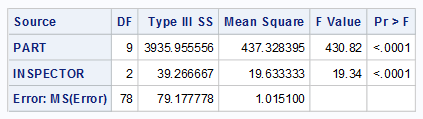
\includegraphics{prob1anova}

I am not familiar with the subject area. This sounds like an observational study, but if inspectors and parts were randomly assigned to induction motor starters, independence between replicates would be reasonable after accounting for inspector and part variability. It is also assumed parts, inspectors, and the residuals are all independent, and all parts are independent, all inspectors are independent, and all residuals are indpendent. These will be reasonable if, for the part, the effect of part 1 does not influence the effect of part 2, and likewise for the residuals and inspectors. Inspectors are human, and so may not be independent if trained in subgroups.

Normality is reasonable as all the residuals fall very close to the normal q-q line. There is one outlier residual near the predicted value of 30. However, it is not too extreme in magnitude and given the number of other residuals, we might expect at least one to be a bit larger by chance. Homogeneity of variance seems reasonable as there is random scatter in the residuals vs. predicted plot.

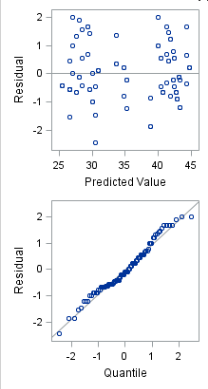
\includegraphics{prob1plots}

\item 

{\it  (1.5pt) Provide estimates of the variance components.}

{\bf ask john what this second plot is}

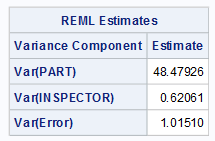
\includegraphics{prob1var}

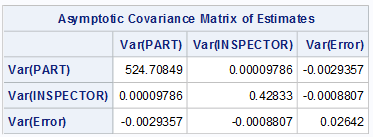
\includegraphics{prob1var1}

\item

{\it (1.5pt) Provide a practical interpretation of the variance component estimates in the context of the study.}

The variation in impedence within {\bf or is it between?} parts is estimated to be 48.47926. The variation in impedence within inspectors is estimated to be 0.62061 and the variation in impedence after accounting for part and  inspector is estimated to be 1.0151.

{\bf fix this up and make sure i understand.}
\end{enumerate}

\item 
{\it (1.5pt) Consider the situation described in Problem 13.7, page 602. Provide estimates of the
variance components.}

{\bf by variance components does he mean mse or all the sums of squares... here it says assume operator is fixed, so really only one variance component...}

\item 
\begin{enumerate}
\item

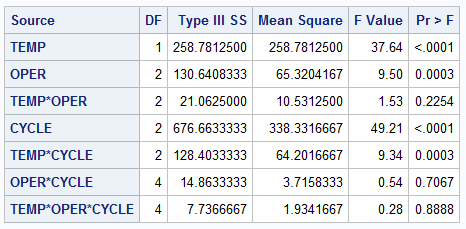
\includegraphics{prob3anova}

\item 

\item

\item %3d

The largest effect occurs at 300 degrees, operator 2, and cycle 50 and so that is my recommendation.

\item 

{\it  (.5pt) If a target score of 30 is desirable, what set of factor conditions would you recommend?}

Want sum of effects to be 0, but not sure how to evaluate.

\item 
{\it  (1pt) Is there any serious problem with the model assumptions? If yes, what is the problem?}

Randomization would make independence of the residuals reasonable. The residuals vs. predicted plot shows random scatter, which suggests constant variance is reasonable. The Normal Q-Q plot shows two residuals that are quite large on the standardized scale and deviate from the normal q-q line, suggesting the normality assumption of the residuals may be violated. Looking a bit closer at the residuals vs. predicted plot we do see two residuals greater than 5 in absolute value near predicted values of 28 ad 35.

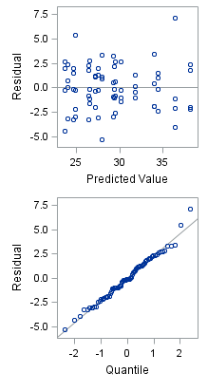
\includegraphics{prob3plots}
\end{enumerate}

\item %4

{\it  Suppose that the data in Problem 3 was not collected as a completely randomized design.
Suppose that two replicates of the three-factor factorial were collected on Monday and the
remaining two replicates of the three-factor factorial were collected on Friday, and that within
each day the 36 experimental runs were completely randomized.}

\begin{enumerate}
\item 

{\it (1.5pt) Describe the model that incorporates the model effects from Problem 2 and additional effects involving Days (Monday, Friday) and all two-factor interactions with Days.}

{\bf Make sure John doesn't want more than main fixed effects.}

\begin{center}
$y_{ijklm} = \mu + \beta_{i} + \gamma_{j} + \phi_{k} + \utilde{\tau}_{l} + \utilde{\beta\tau}_{il} + \utilde{\gamma\tau}_{jl} + \utilde{\phi\tau}_{kl} + \utilde{\epsilon}_{ijklm}$
\end{center}

where i = level of temperature (1,2)

j = operator level (1,2,3)

k = cycle level (1,2,3)

l = day (1,2)

m = replicate (1,2)

\item 
{\it  (1.5pt) Set up a partial ANOVA table with a column for the Source of Variation. This will include rows that corresponding to the model effects in (a) as well as rows for Error and Total. Include a second column with the associated degrees of freedom. No data analysis is needed.}

\begin{center}
\begin{tabular}{|l|l|l|}
Source & df\\
temp & 1\\
oper & 2\\
cycle & 2\\
day & 1\\
temp*day & 1\\
oper*day & 2\\
cycle*day & 2\\
error & 60\\
total & 71
\end{tabular}
\end{center}

\item 
{\it  (1pt) Typically, the MSE represents an estimate of $\sigma^{2}$. For this to be true, we will need to assume all other potential model effects are negligible and can be ignored. What potential model effects did we assume to be negligible and exclude from the model?}

The model effects we assumed to be negligible and excluded from the model include $\beta\gamma_{ij}$, $\beta\phi_{ik}$, $\gamma\phi_{jk}$, $\beta\gamma\phi_{ijk}$, $\utilde{\tau\beta\gamma}_{ijl}$, $\utilde{\tau\beta\phi}_{ikl}$, $\utilde{\tau\gamma\phi}_{jkl}$, $\utilde{\tau\beta\gamma\phi}_{ijkl}$.

\end{enumerate}

\item 

{\it Consider the information on pages 192-194 for Example 5.1 for the battery design experiment.
Suppose the researcher is planning another 3�3 factorial experiment. The goal is to determine
the sample size required so that the power of each F-test (for Material Type, Temperature,
and their interaction) is $\geq$ .90.}
\begin{enumerate}
\item
{\it  (.5pt) Based on this experiment, what is the estimate of $\sigma$?}

MSE=675.1 and RMSE=$\hat{\sigma}$=25.9826865.

\itwm
{\it  (1.5pt) Determine the desired sample size assuming you use the sample mean $y_{ij}$ as an estimate of $\mu$ij for i = 1, 2, 3 and j = 1, 2, 3. You can assume $\alpha$= .05.}

The computed total sample size is 18, meaning two replicates per each material and temperature combination.

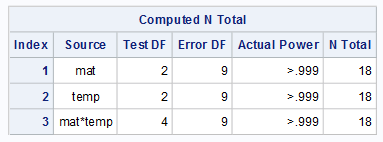
\includegraphics{prob5power}

\begin{verbatim}
DATA p5;
 DO mat = 1 TO 3;
   DO temp = 1 to 3;
      INPUT life @@; OUTPUT;
   END; END;
 LINES;
 539 229 230
 623 479 198
 576 583 342
;
PROC GLMPOWER DATA = p5;
CLASS mat temp;
MODEL life=mat|temp;
POWER
STDDEV = 25.98269
ALPHA = 0.05
NTOTAL = .
POWER = 0.9;
RUN;
\end{verbatim}

\end{enumerate}

\item
{\it Stat 541 students: Suppose that the data in Problem 3 was not collected as a completely randomized design. Suppose that one replicate of the three-factor factorial was collected on Monday, Tuesday, Thursday, and Friday, and that within each of these four days, the 18 experimental runs were completely randomized.}

\begin{enumerate}
\item

{\it (3pt) For a model that incorporates model effects involving Days, Temperature, Operator,
and Cycle Time, as well as all two-factor and three-factor interactions involving
Temperature, Operator, Cycle Time, and Days, set up a partial ANOVA table that
includes these model effects and the associated degrees of freedom.}

\begin{center}
\begin{tabular}{|l|l|l|}
Source & df\\
temp & 1\\
oper & 2\\
cycle & 2\\
day & 3\\
temp*day & 3\\
oper*day & 6\\
cycle*day & 6\\
temp*oper & 2\\
temp*cycle & 2\\
oper*cycle & 4\\
temp*oper*cycle & 4\\
temp*day*oper & 6\\
temp*day*cycle & 6\\
day*oper*cycle & 12\\
error & 12\\
total & 71
\end{tabular}
\end{center}

\item 
{\it  (1pt) What does the MSE actually estimate in the context of this study?}

In this study, the MSE is actually the four way interaction between temperature, day, operator, and cycle time because there is no replication.
\end{enumerate}
\end{enumerate}


\end{document}
